\chapter{Mod�le du syst�me}
%          * Cas d'utilisation (diagrammes UML)
%          * Mod�le abstrait de donn�es (diagrammes UML) 

Dans  cette partie, nous  �tudierons tout  d'abord les  diff�rents cas
d'utilisation du  logiciel.

\section{Vue g�n�rale de \visidia}
Voici tout d'abord une repr�sentation simplifi�e du diagramme des cas
d'utilisation sur la figure \ref{fig:cu_vue_generale}. Nous nous
int�resserons dans la suite de ce document uniquement au cas
d'utilisation \textbf{Simuler un calcul distribu� bas� sur des agents}
(\ref{fig:cu_simuler}).


\begin{figure}[H]
  \centering
  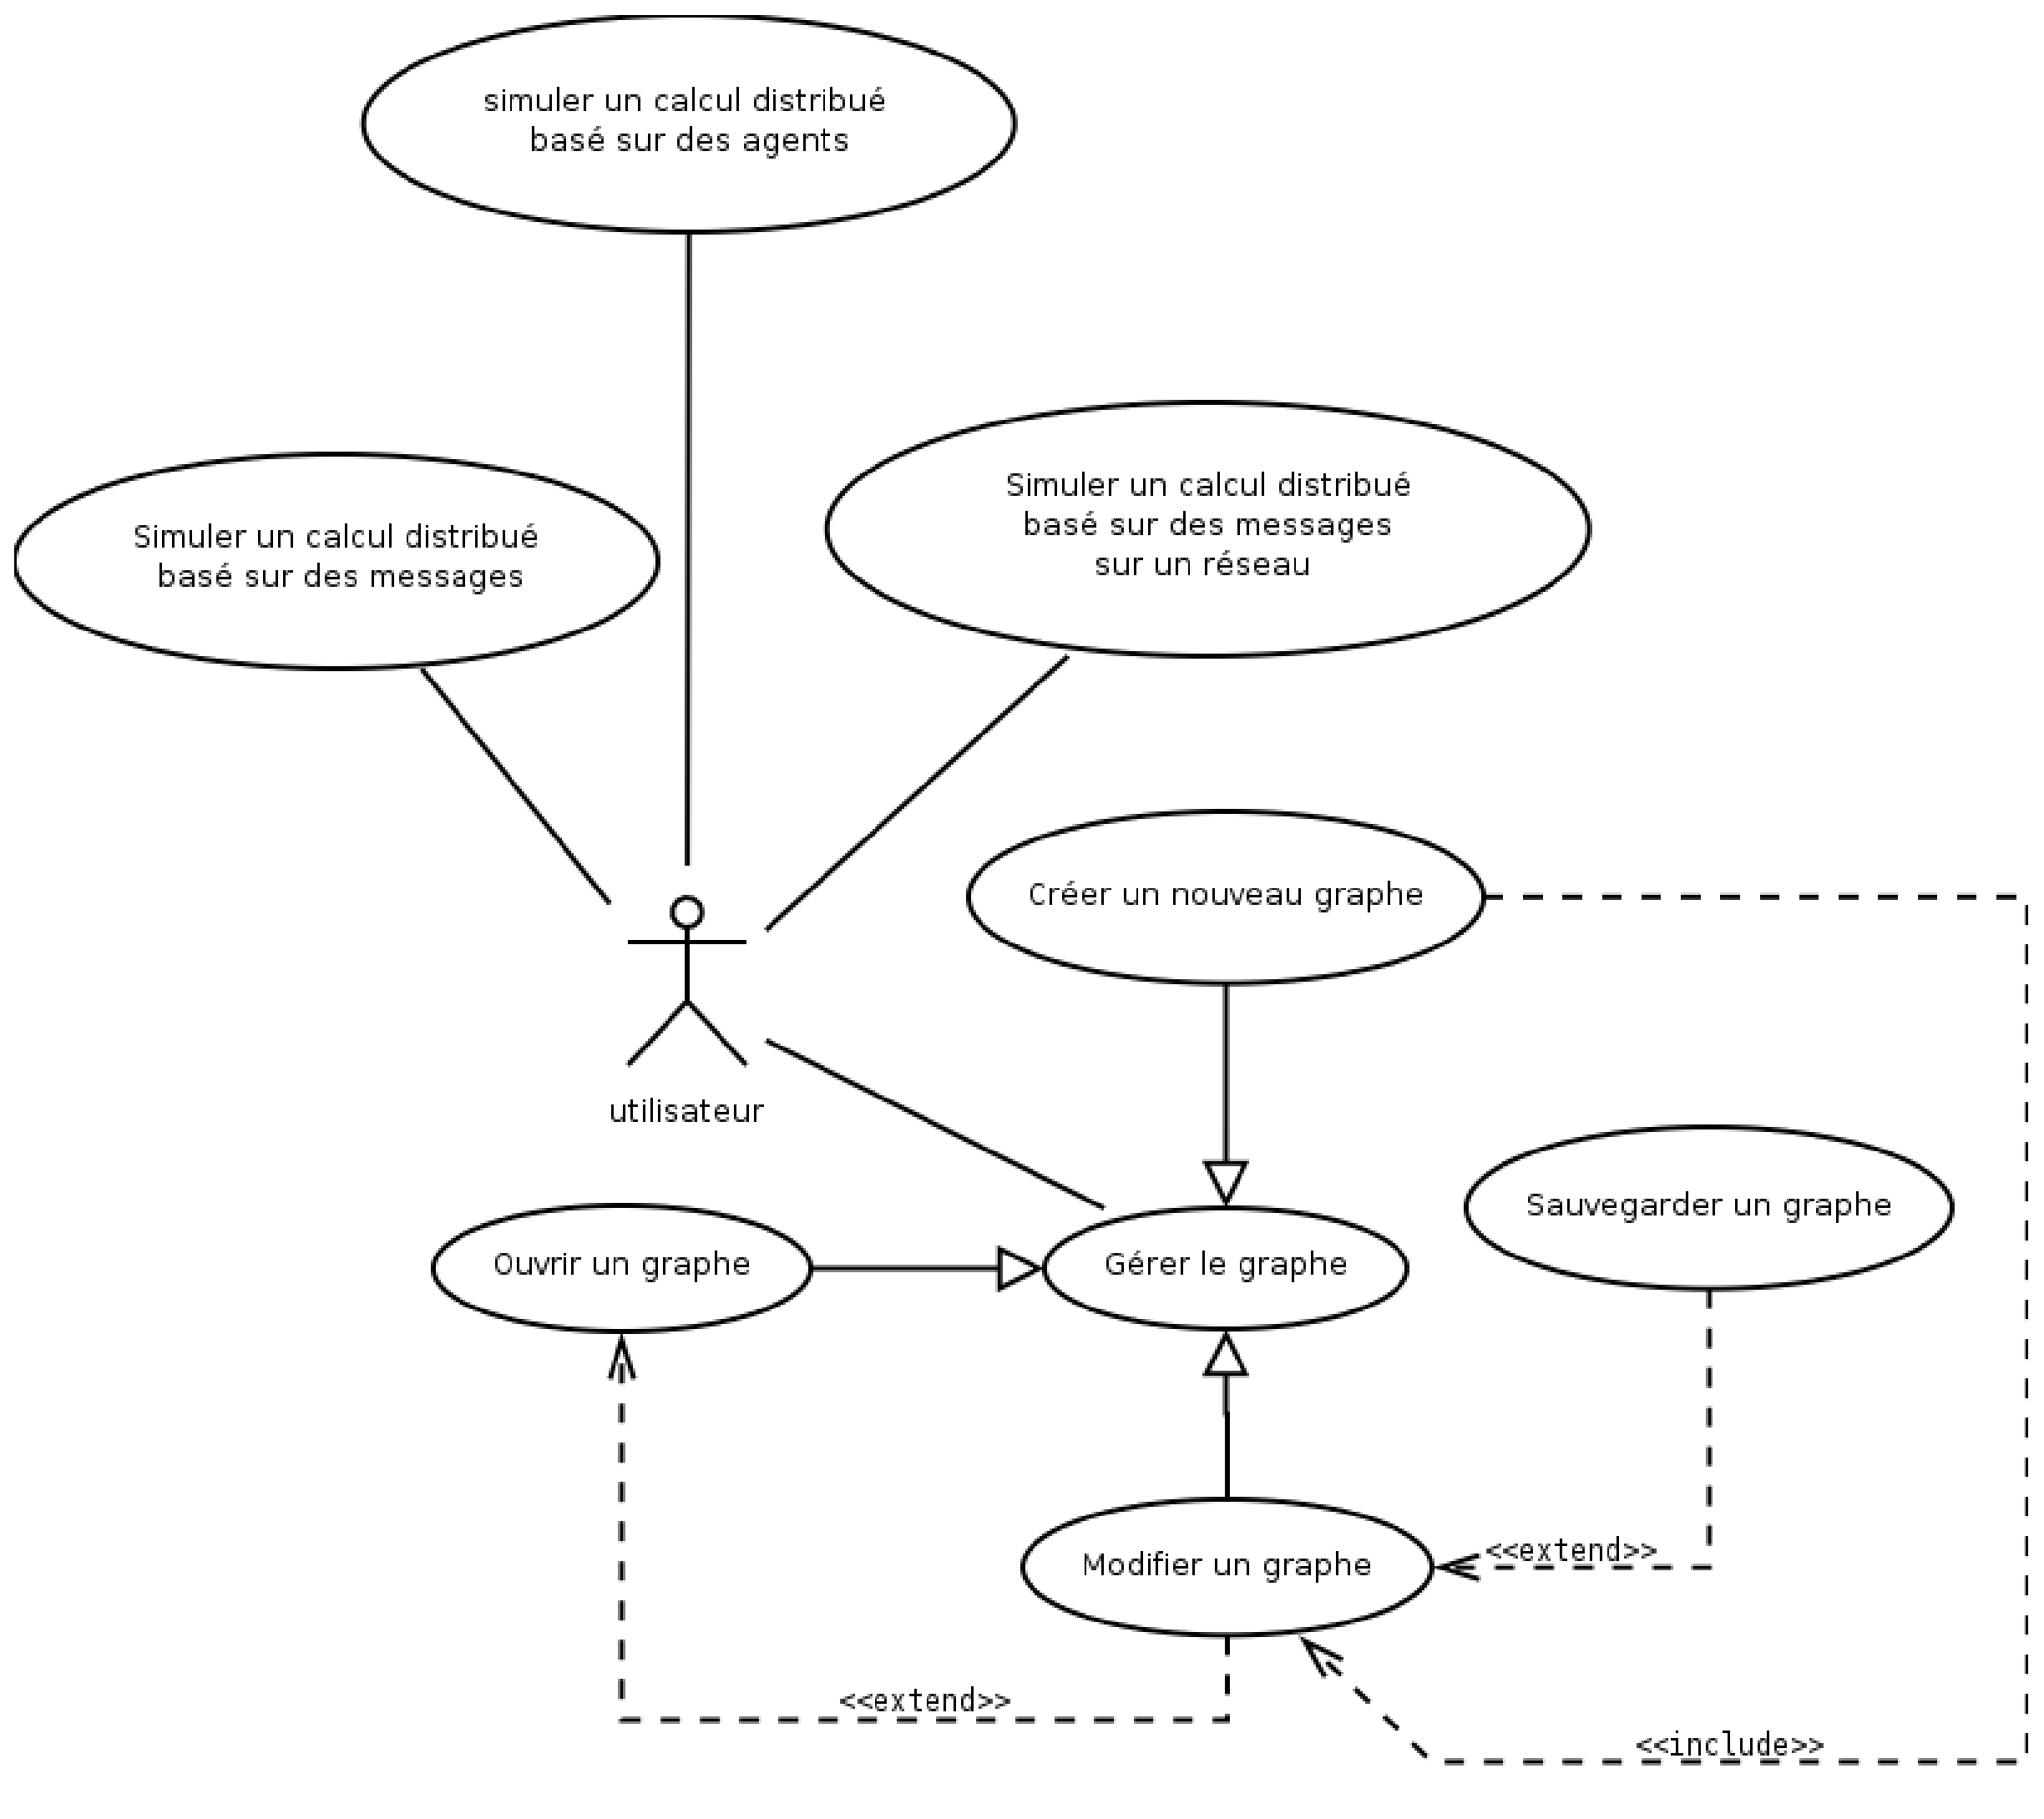
\includegraphics[width=14cm]{img/visidia_cu_vue_generale}
  \caption{Cas d'utilisation : Vue g�n�rale de \visidia} 
  \label{fig:cu_vue_generale}
\end{figure}

\begin{figure}[H]
  \centering
  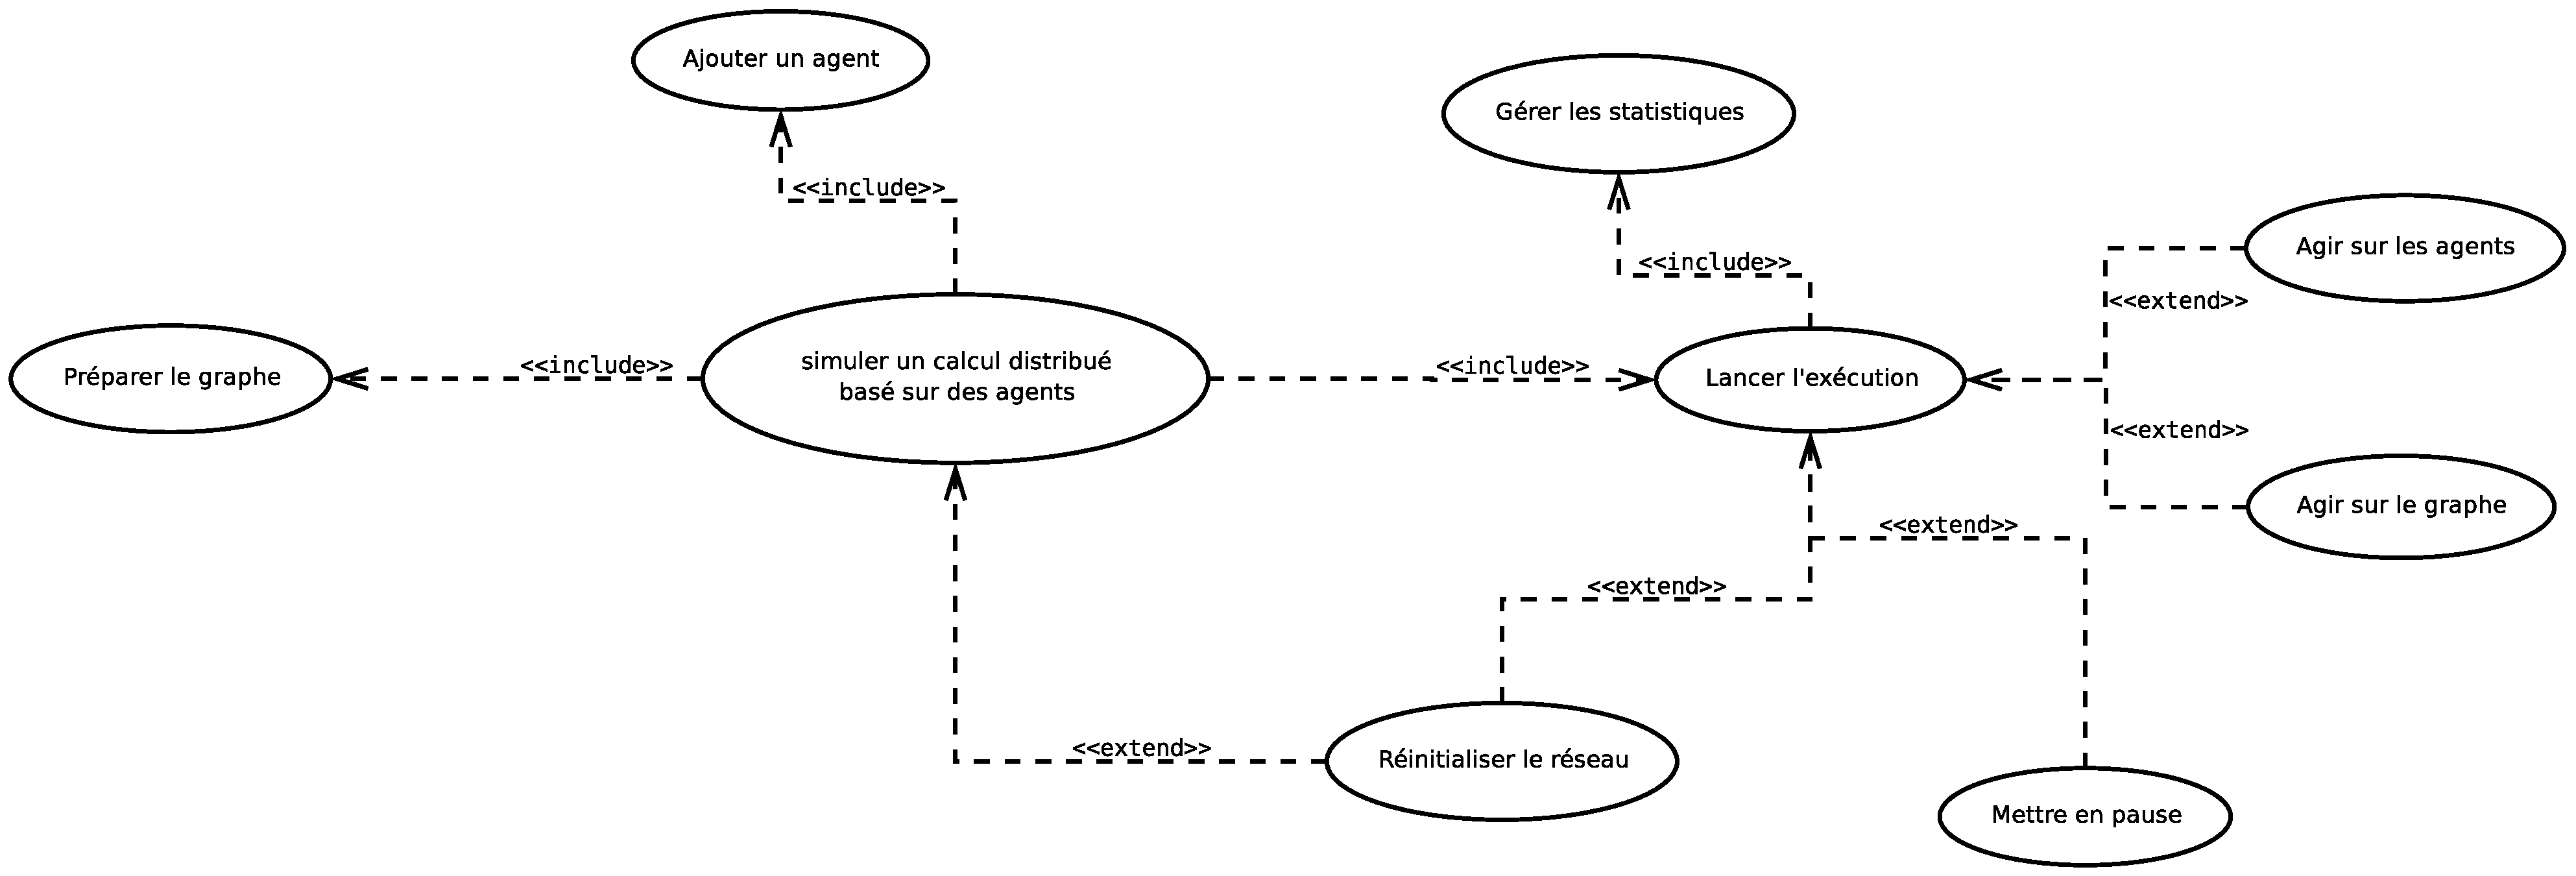
\includegraphics[width=24cm,angle=90]{img/visidia_cu_simuler_agent}
  \caption{Cas d'utilisation : Simuler agent} 
  \label{fig:cu_simuler}
\end{figure}

\begin{figure}[H]
  \centering
  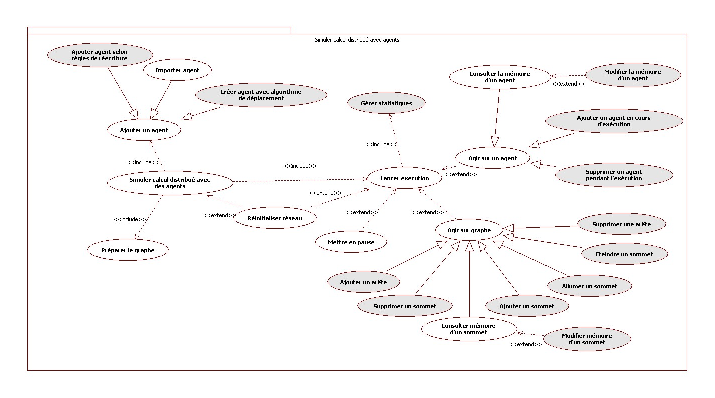
\includegraphics[width=24cm,angle=90]{img/visidia_cu_simuler_agent_all.eps}
  \caption{Cas d'utilisation :  Simuler agent \visidia (d�taill�)} 
  \label{fig:cu_simuler_agent_all}
\end{figure}

\section{Description des cas d'utilisation}
\subsection{Ajout d'un agent}

\begin{figure}[H]
  \centering
  
\includegraphics[width=14cm]{img/visidia_cu_ajouter_agent}
  \caption{Cas d'utilisation : Ajouter un agent} 
  \label{fig:cu_ajouter_agent}
\end{figure}

%%%%%%%%%%%%%%%%%%%
%%% � commenter %%%
%%%%%%%%%%%%%%%%%%%

\subsection{Actions sur les agents}

\begin{figure}[H]
  \centering
  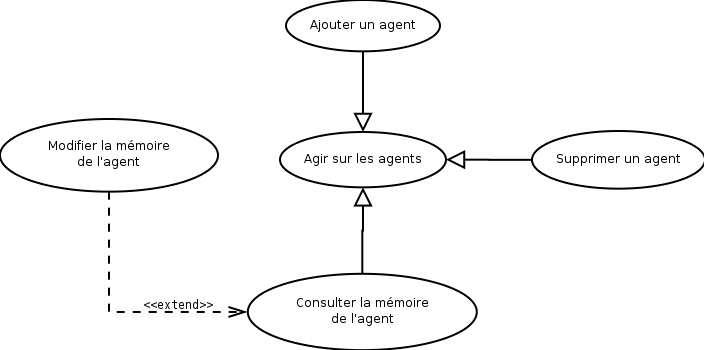
\includegraphics[width=14cm]{img/visidia_cu_agir_agent}
  \caption{Cas d'utilisation : Agir sur un agent} 
  \label{fig:cu_agir_agent}
\end{figure}

\subsubsection {Supprimer un agent}
Ce cas d'utilisation va permettre � l'utilisateur de supprimer un agent d'un r�seau lors de l'�xecution d'un algorithme.

\begin{tabular}{|l|l|}
\hline
Cas d'utilisation 	& Supprimer un agent. \\
\hline
Acteur 			& L'utilisateur. \\
\hline 
But 			& Supprimer un agent du r�seau au moment de l'�xecution d'un algoritme. \\
\hline
R�sum� M�tier 		& L'utilisateur choisit un agent pour le supprimer.\\
\hline
Pr� conditions 		& L'utilisateur dispose d'un agent dans le r�seau. \\
 \hline
Post conditions 	& L'agent n'est plus dans le r�seau.\\
\hline
Commentaires 		& On ne peut supprimer qu'un seul agent � la fois.\\
\hline
\end{tabular}


\subsubsection {Ajouter un agent}
Ce cas d'utilisation va permettre � l'utilisateur d'ajouter un agent sur un sommet (non eteint) de r�seau.

\begin{tabular}{|l|l|}
\hline
Cas d'utilisation 	& Ajouter un agent. \\
\hline
Acteur 			& L'utilisateur. \\
\hline 
But           		& Ajouter un agent dans un r�seau au moment de l'�xecution d'un tel algoritme. \\
\hline

R�sum� M�tier 		& L'utilisateur choisit un sommet, il choisit un agent parmi les agents qu'on a, puis il l'ajoute.\\
\hline
Pr� conditions 		& L'utilisateur dispose d'un r�seau et d'une implantation d'agent. \\
 \hline
Post conditions 	& L'agent est bien ajout� sur une sommet.\\
\hline
Commentaires 		& On ne peut ajouter qu'un seul agent � la fois.\\
\hline
\end{tabular}

\subsubsection {Consulter un agent}
Ce cas d'utilisation va permettre � l'utilisateur de consulter la m�moire d'un agent. 

\begin{tabular}{|l|l|}
\hline
Cas d'utilisation 	& consulter un agent. \\
\hline
Acteur 			& L'utilisateur. \\
\hline 
But 			& Consulter un agent dans un r�seau au moment de l'�xecution d'un algoritme. \\
\hline
R�sum� M�tier 		& L'utilisateur choisit un agent puis le consulte.\\
\hline
Pr� conditions 		& L'utilisateur dispose d'un r�seau et d'une implantation d'agent. \\
 \hline
Post conditions 	& L'agent est bien ajout� sur une sommet.\\
\hline
Commentaires 		& On ne peut consulter qu'un seul agent � la fois.\\
\hline
\end{tabular}


\subsubsection {Modifier la m�moire d'un agent}
Ce cas d'utilisation va permettre � l'utilisateur de modifier la m�moire d'un agent afin d'agir sur l'�xecution de l'agorithme sur le r�seau.\\


\begin{tabular}{|l|l|}
\hline
Cas d'utilisation 	& Modifier la m�moire f'un agent. \\
\hline
Acteur 			& L'utilisateur. \\
\hline 
But 			& Modifier la m�moire d'un agent dans un r�seau au moment de l'�xecution d'un algoritme. \\
\hline
R�sum� M�tier 		& L'utilisateur choisit un agent puis il modifie sa m�moire.\\ 
\hline
Pr� conditions 		& L'utilisateur dispose d'un agent dans le r�seau. \\
 \hline
Post conditions 	& La m�moire de l'agent est bien modifi�.\\
\hline
Commentaires 		& On peut modifier la m�moire que d'un seul agent � la fois.\\
\hline
\end{tabular}

\subsection{Action sur le graphe}

\begin{tabular}{|c|c|}
\hline
{Cas d'utilisation}    & ........ \\ \hline
{Acteur}    & ........ \\ \hline
{But}    & ........ \\ \hline
{R�sum� m�tier}    & ........ \\ \hline
{Pr� condition}    & ........ \\ \hline
{Post condition}    & ........ \\ \hline
{Commentaires}    & ........ \\ \hline
\caption{........}
\hline
\end{tabular}



\paragraph*{Modifier la m�moire d'un sommet}
Ce cas d'utilisation va permettre � l'utilisateur de modifier la memoire d'un sommet c'est a dire les variables declarees et l'etat
des ports.


\begin{tabular}{|c|c|}
\hline
{Cas d'utilisation}   & Modifier la m�moire d'un sommet. \\ \hline
{Acteur}              & L'utilisateur. \\ \hline
{But}                 & Permettre � l'utilisateur d'agir sur un sommet pour le modifier. \\ \hline
{R�sum� m�tier}       & L'utilisateur choisit un sommet et modifie son whiteboard selon ses besoins. \\ \hline
{Pr� condition}       & L'utilisateur s�lectionne le sommet � modifier.\\ \hline
{Post condition}      & La m�moire du sommet s�lectionn� est modifi�e. \\ \hline
{Commentaires}        & On ne peut modifier qu'un seul sommet � la fois.\\ \hline
\hline
\end{tabular}



\paragraph*{Eteindre un sommet}
Ce cas d'utilisation va permettre � l'utilisateur d'�teindre un sommet 
sans pour autant le supprimer. 

\begin{tabular}{|c|c|}
\hline
{Cas d'utilisation}  & Eteindre un sommet. \\ \hline
{Acteur}             & L'utisateur. \\ \hline
{But}                & Permettre � l'utilisateur d'�teindre un sommet de son choix. \\ \hline
{R�sum� m�tier}      & L'utilisateur choisit un sommet et l'�teint. \\ \hline
{Pr� condition}      & L'utilisateur s�lectionne le sommet (qui doit etre allume) � �teindre. \\ \hline
{Post condition}     & Le sommet s�lectionn� est �teint. \\ \hline
{Commentaires}       & On ne peut �teindre qu'un seul sommet � la fois.\\ \hline
\hline
\end{tabular} 

\begin{tabular}{|c|c|}
\hline
{Numero enchainement}    & Action \\ \hline
{1}    & L'utilisateur choisit un sommet a eteindre n'hebergeant pas d'agent. \\ \hline
{2}    & Le systeme eteint le sommet. \\ \hline
\hline
\end{tabular}


\begin{tabular}{|c|c|}
\hline
{Numero enchainement}    & Action \\ \hline
{1}    & L'utilisateur choisit un sommet a eteindre hebergeant un agent. \\ \hline
{2}    & ??????????????????????????????????????????????????????? \\ \hline
{3}    & Le systeme eteint le sommet. \\ \hline
\hline
\end{tabular}

?????????????????????????????/ Agent aur arete
eteindre : garder la memoire ou pas???????????



\paragraph*{Consulter un sommet}
Ce cas d'utilisation va permettre � l'utilisateur de consulter la m�moire d'un sommet.

\begin{tabular}{|c|c|}
\hline
{Cas d'utilisation}  & Consulter un sommet. \\ \hline
{Acteur}             & L'utilisateur. \\ \hline
{But}                & Permettre � l'utilisateur de consulter la m�moire d'un sommet. \\ \hline
{R�sum� m�tier}      & L'utilisateur choisit selon ses besoins un sommet et consulte sa memoire. \\ \hline
{Pr� condition}      & L'utilisateur s�lectionne le sommet � consulter. \\ \hline
{Post condition}     & Le sommet s�lectionn� est consult�. \\ \hline
{Commentaires}       & On ne peut consulter que la m�moire d'un seul sommet � la fois. \\ \hline
\hline
\end{tabular}




\paragraph*{Allumer un sommet}
Ce cas d'utilisation va permettre � l'utilisateur d'allumer un sommet. 
Ce dernier doit �tre d�j� �teint car allumer un sommet qui n'est pas 
�teint n'a pas de sens.

\begin{tabular}{|c|c|}
\hline
{Cas d'utilisation}  & Allumer un sommet.  \\ \hline
{Acteur}             & L'utilisateur. \\ \hline
{But}                & Permettre � l'utilisateur d'allumer un sommet. \\ \hline
{R�sum� m�tier}      & L'utilisateur choisit selon ses besoins un sommet et l'allume. \\ \hline
{Pr� condition}      & L'utilisateur s�lectionne le sommet � allumer. Ce sommet doit �tre d�j� �teint. \\ \hline
{Post condition}     & Le sommet s�lectionn� est allum�.  \\ \hline
{Commentaires}       & On ne peut allumer qu'un seul sommet(�teind) � la fois.  \\ \hline
\hline
\end{tabular}





\subsubsection{Ajouter un sommet pendant l'ex�cution}

\begin{tabular}{|l|p{10cm}|}
\hline
{Cas d'utilisation}    & Ajouter un sommet pendant l'ex�cution\\ \hline
{Acteur}               & L'utilisateur \\ \hline
{But}                  & Ajouter un sommet dans le graphe pendant une ex�cution \\ \hline
{R�sum� m�tier}        & L'utilisateur indique dans la fen�tre de simulation l'endroit o� ajouter un sommet \\ \hline
{Pr�-condition}        & L'utilisateur dispose d'un graphe en cours d'ex�cution \\ \hline
{Post-condition}       & Le sommet est ajout� au graphe \\ \hline
{Commentaires}         & Le sommet n'est pas connect� au graphe \\ \hline
\end{tabular}



\subsubsection{Supprimer un sommet pendant l'ex�cution}

\begin{tabular}{|l|p{10cm}|}
\hline
{Cas d'utilisation}    & Supprimer un sommet pendant l'ex�cution\\ \hline
{Acteur}               & L'utilisateur \\ \hline
{But}                  & Ajouter un sommet dans le graphe pendant une ex�cution \\ \hline
{R�sum� m�tier}        & L'utilisateur indique dans la fen�tre de simulation le sommet � supprimer \\ \hline
{Pr�-condition}        & L'utilisateur dispose d'un graphe en cours d'ex�cution \\ \hline
{Post-condition}       & Le sommet et toute ar�te incidente � celui-ci est supprim�e (voir cas d'utilisation supprimer ar�te) \\ \hline
{Commentaires}         & Il n'y a pas de notification du crash aux voisins. Les agents �ventuellement pr�sents sur le sommet sont supprim�s \\ \hline
\end{tabular}


\subsubsection{Ajouter une ar�te pendant l'ex�cution}

\begin{tabular}{|l|p{10cm}|}
\hline
{Cas d'utilisation}    & Ajouter une ar�te pendant l'ex�cution \\ \hline
{Acteur}               & L'utilisateur \\ \hline
{But}                  & Ajouter une ar�te dans le graphe pendant une ex�cution \\ \hline
{R�sum� m�tier}        & L'utilisateur indique les deux sommets distincts � connecter et qui ne sont pas encore connect�s \\ \hline
{Pr�-condition}        & L'utilisateur dispose d'un graphe en cours d'ex�cution \\ \hline
{Post-condition}       & L'ar�te est ajout�e, \\
                       & les deux sommets � connecter prennent compte la nouvelle ar�te\\
		       & et l'ex�cution se poursuit \\ \hline
{Commentaires}         & Lors de l'ajout d'une ar�te, l'ex�cution est mise en pause \\ \hline
\end{tabular}




\subsubsection{Supprimer une ar�te pendant l'ex�cution}

\begin{tabular}{|l|p{10cm}|}
\hline
{Cas d'utilisation}    & Supprimer une ar�te pendant l'ex�cution \\ \hline
{Acteur}               & L'utilisateur \\ \hline
{But}                  & Supprimer une ar�te dans le graphe pendant une ex�cution \\ \hline
{R�sum� m�tier}        & L'utilisateur indique l'ar�te � supprimer \\ \hline
{Pr�-condition}        & L'utilisateur dispose d'un graphe en cours d'ex�cution \\ \hline
{Post-condition}       & L'ar�te est supprim�e, les deux sommets reli�s par cette ar�te prennent en compte sa suppression \\ \hline
{Commentaires}         & Lors de la suppression d'une ar�te,
                         l'ex�cution est mise en pause.\\
                       & Les agents �ventuellement pr�sents sur l'ar�te � supprimer sont supprim�s \\
 \hline 
\end{tabular}


\subsection{Statistiques}

\subsubsection{Afficher des statistiques par agent}
Ce cas d'utilisation va permettre � l'utilisateur d'afficher des statisques pour un agent donn� � la fin de l'algorithme.


\begin{tabular}{|l|l|}
\hline
{Cas d'utilisation}   & Afficher les statistiques d'un agent \\ \hline
{Acteur}              & L'utilisateur. \\ \hline
{But}                 & Permettre � l'utilisateur de voir les statistiques d'un agent donn�. \\ \hline
{R�sum� m�tier}       & L'utilisateur s�lectionne un agent et voit ses statistiques : le nombre de pas qu'il a fait entre le d�but et la fin de l'ex�cution del'algorithme, l'evolution de la taille de la memoire de sa m�moire .\\ \hline
{Pr� condition}       & L'utilisateur s�lectionne un agent.\\ \hline
{Post condition}      & Les statistiques sur l'agent sont affich�s. \\ \hline
{Commentaires}        & \\ \hline
\end{tabular}



\subsubsection{Afficher des statistiques sur l'execution d'un algorithme}
Ce cas d'utilisation va permettre � l'utilisateur d'afficher des statisques sur un algorithme � la fin de son execution.

\begin{tabular}{|l|l|}
\hline
{Cas d'utilisation}  & Afficher les statistiques sur l'execution d'un algorithme \\ \hline
{Acteur}             & L'utisateur. \\ \hline
{But}                & Permettre � l'utilisateur de voir les statistiques de l�execution d'un algorithme \\ \hline
{R�sum� m�tier}      & L'utilisateur selectionne l'option ``afficher statistiques'' et consulte les informations suivantes : cout de l'algorithme( somme des pats des agents), temps de l'algorithme (max(nombre pas des agents)), nombre max d'agents au cours de l'execution.\\ \hline
{Pr� condition}      & L'algorithme a fini de s'executer \\ \hline
{Post condition}     & Les statistiques sont calcul�s et s'affichent \\ \hline
{Commentaires}       & \hline
\end{tabular} 


\section{Diagramme de classes}

Nous reprenons l'architecture du projet \visidia existant et  nous
nous  contenterons d'apporter les fonctionnalit�s n�cessaires au
programme. Nous rappelons ci-dessous le diagramme de classe  existant
l�g�rement modifi� par l'ajout de certaines fonctionnalit�s.

\begin{figure}[H]
  \centering
  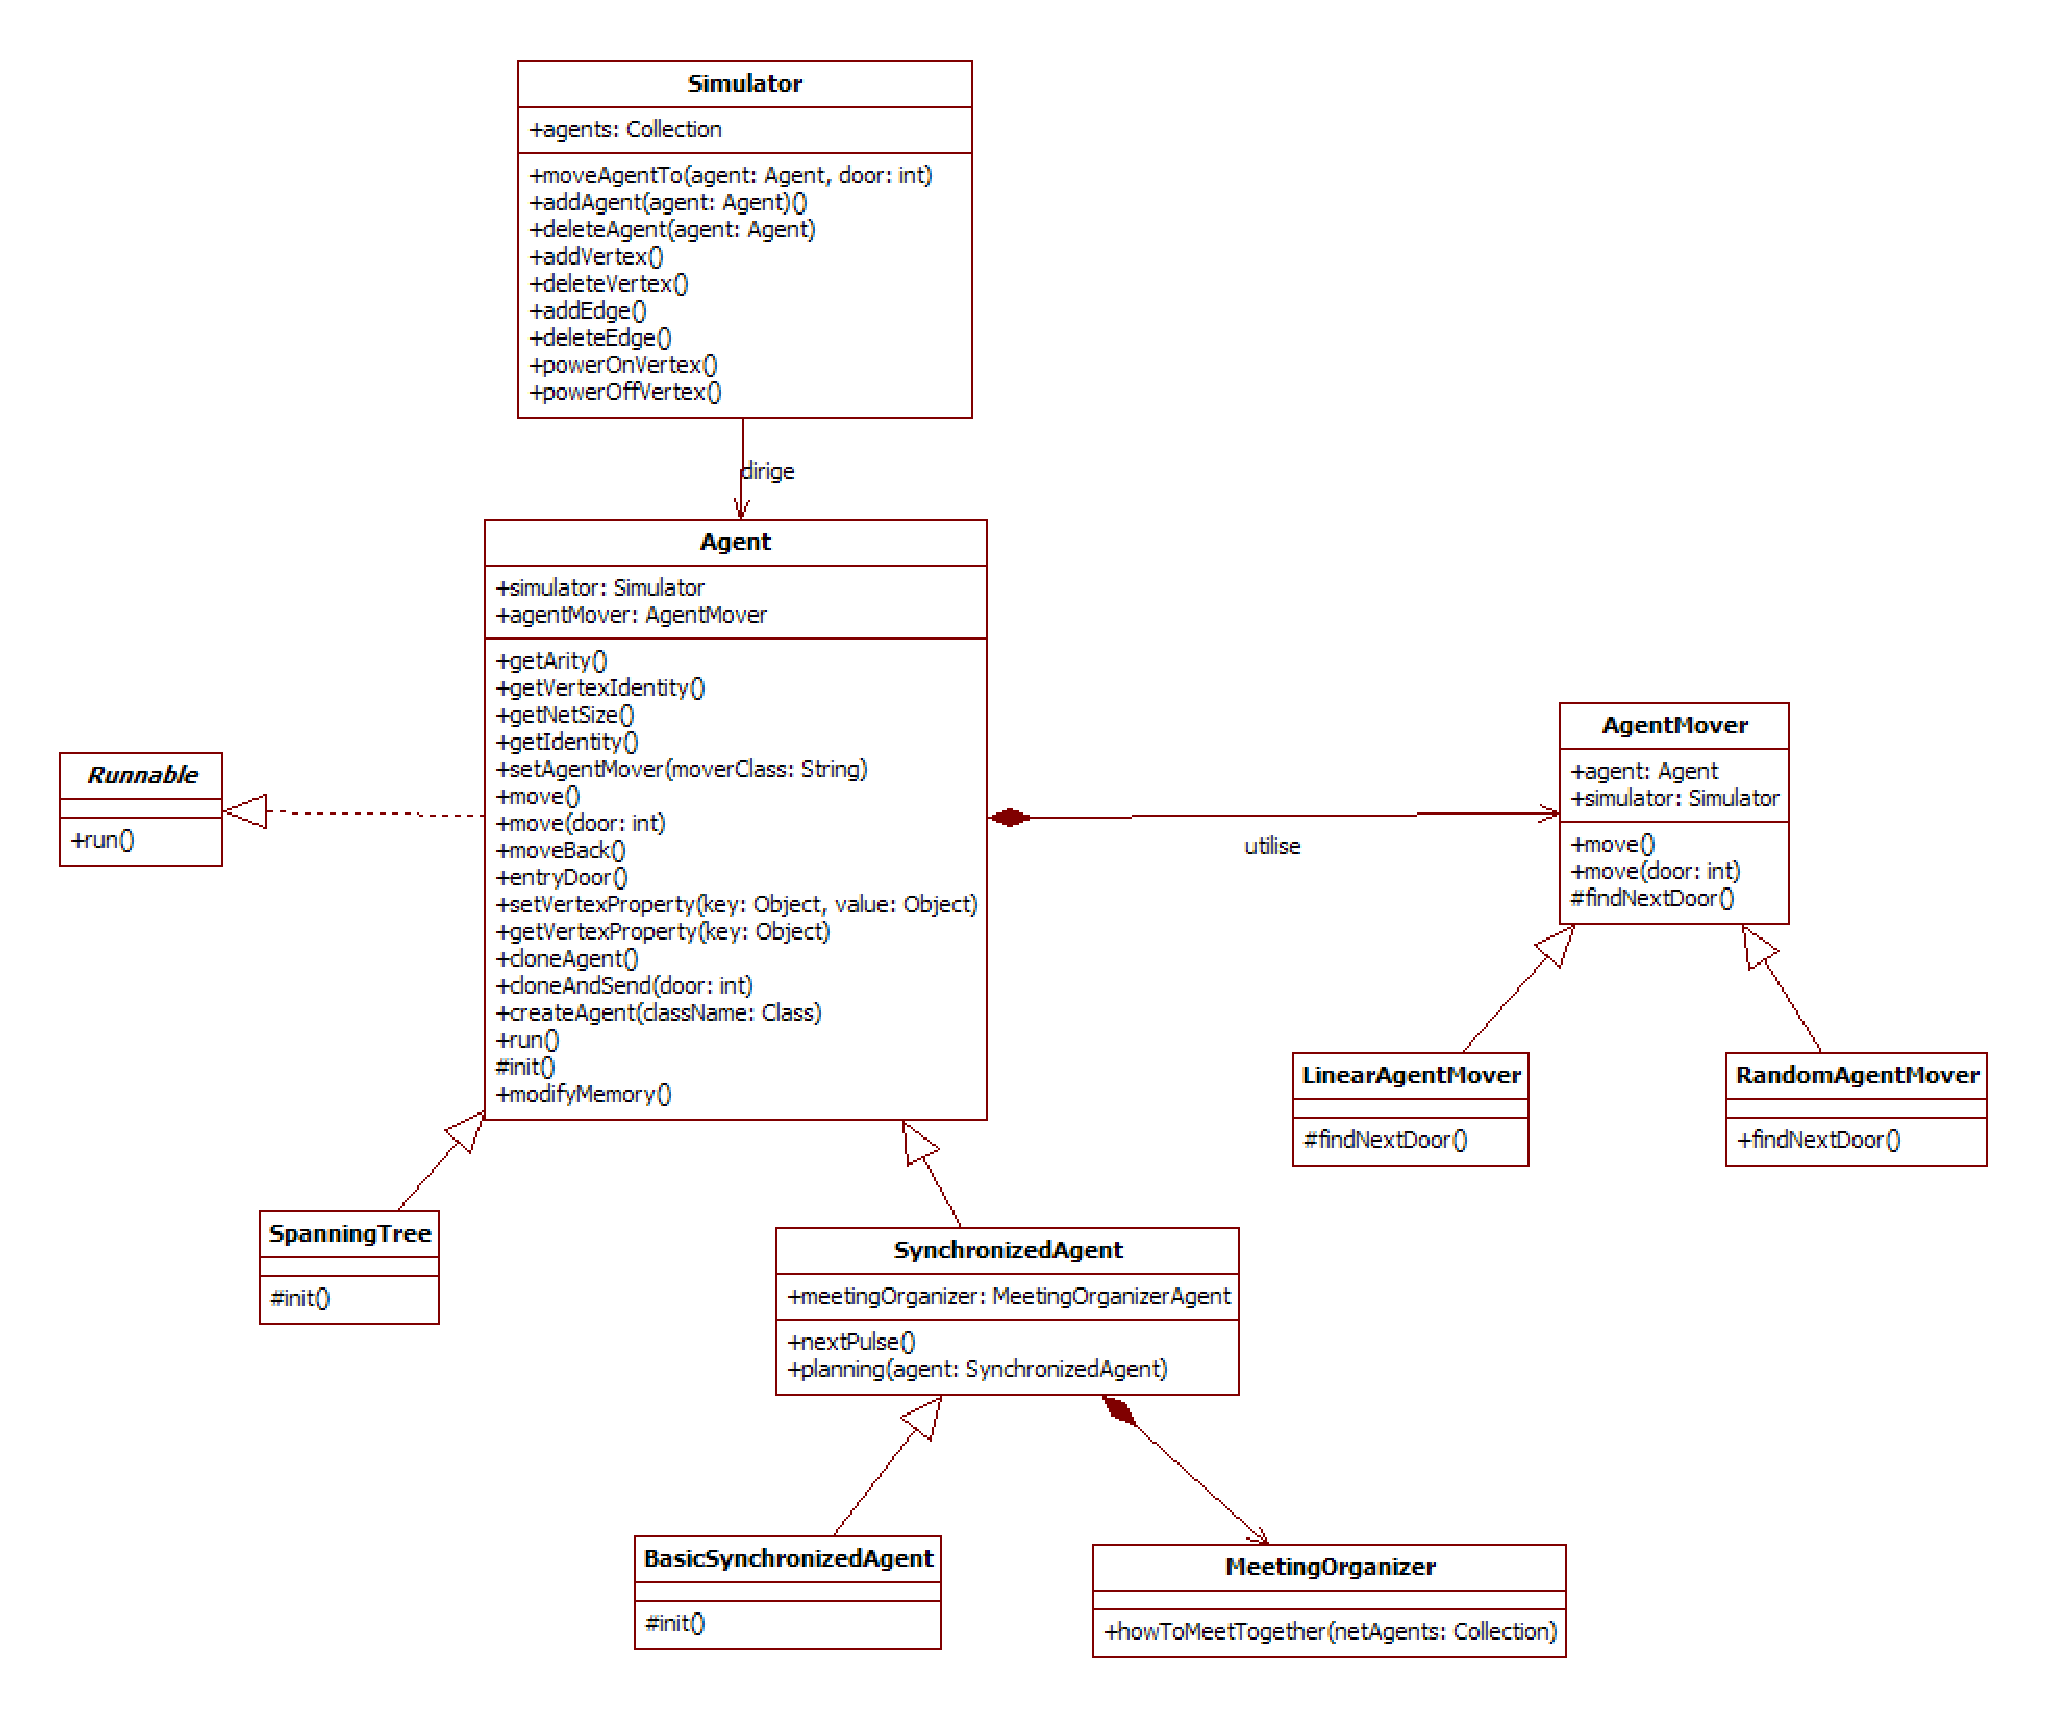
\includegraphics[width=14cm]{img/ImagesJu/ClassDiagram1}
  \caption{Diagramme de classes candidates}
  \label{fig:cu_ajouter_agent}
\end{figure}


\section{Diagramme de s�quences}

Nous donnons ci-dessous un diagramme de s�quence correspondant �
un sc�nario nominal d'utilisation du logiciel \visidia, avec
cr�ation d'un graphe, ajout d'un agent, ex�cution et simulation,
modification du graphe, affichage de statistiques et arr�t de la simulation.

\begin{figure}[H]
  \centering
  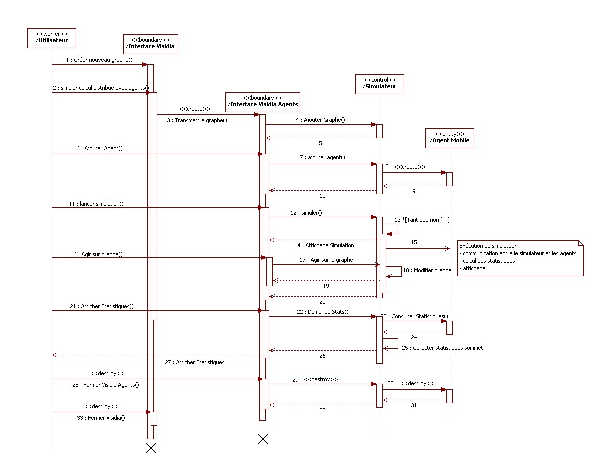
\includegraphics[width=14cm]{img/DiagrammeSequence}
  \caption{Diagramme de s�quences} 
  \label{fig:cu_ajouter_agent}
\end{figure}









